\documentclass[12pt]{article}
\usepackage[utf8]{inputenc}
\usepackage{polski}
\usepackage{alltt}
\usepackage{float}
\usepackage[a4paper, total={6in, 10in}]{geometry}
\usepackage{listings}
\usepackage{xcolor}
\usepackage{systeme}
\usepackage[usestackEOL]{stackengine}
\usepackage{natbib}
\usepackage{graphicx}
\usepackage{amsmath}
\usepackage{listings}
\usepackage{color} %red, green, blue, yellow, cyan, magenta, black, white
\definecolor{mygreen}{RGB}{28,172,0} % color values Red, Green, Blue
\definecolor{mylilas}{RGB}{170,55,241}
\newcommand{\norm}[1]{\left\lVert#1\right\rVert}
\usepackage{subfigure}
\usepackage{subfig}
\usepackage{minted}


\begin{document}


\lstset{language=Matlab,%
    %basicstyle=\color{red},
    breaklines=true,%
    morekeywords={matlab2tikz},
    keywordstyle=\color{blue},%
    morekeywords=[2]{1}, keywordstyle=[2]{\color{black}},
    identifierstyle=\color{black},%
    stringstyle=\color{mylilas},
    commentstyle=\color{mygreen},%
    showstringspaces=false,%without this there will be a symbol in the places where there is a space
    numbers=left,%
    numberstyle={\tiny \color{black}},% size of the numbers
    numbersep=9pt, % this defines how far the numbers are from the text
    emph=[1]{for,end,break,function},emphstyle=[1]\color{red}, %some words to emphasise
    %emph=[2]{word1,word2}, emphstyle=[2]{style},    
}

\thispagestyle{empty}
\begin{flushright}{\large Rzeszów, 20.10.2021 }
\end{flushright}
\vspace{1.5cm}
\vspace{4.5cm}
\begin{center}
{\large
PODSTAWY MODELOWANIA MATEMATYCZNEGO W INŻYNIERII\par\vspace{2cm}\par
PRACA LABORATORYJNA NR 2\par\vspace{0.2cm}\par
"Modele matematyczne w postaci układów równań
różniczkowych zwyczajnych i metody ich rozwiązania."\par\vspace{0.2cm}\par
}

\end{center}
\vspace{8cm}

{\raggedleft\vfill\Longstack[l]{%
  \large Piotr Krawiec L1\vspace{0.2cm} \\
  \large Semestr: 2021/2022 \vspace{0.2cm} \\
  \large Kierunek: III/FS0-DI \vspace{0.2cm} \\
  \large Numer indeksu: 164165 \vspace{0.2cm} \\
  \large Prowadzący: Bohdan Datsko
}\par
}
\vfill


\leavevmode\thispagestyle{empty}\newpage

\section{Treść zadania}
Wykonać modelowanie różnych możliwych typów zachowań
układów oscylacyjnych przedstawionych na rysunkach \ref{schemat1} i \ref{schemat2}. Innymi słowy,
otrzymać różne typy rozwiązań układów równań różniczkowych dla
parametrów podanych w tabeli 2 zgodnie z zestawem. Ocenić skuteczność
obliczeń i użytych metod numerycznych i analitycznych.

\subsection{Badane układy i funkcje}
\begin{figure}[H]
  \centering
  \begin{minipage}[b]{0.4\textwidth}
    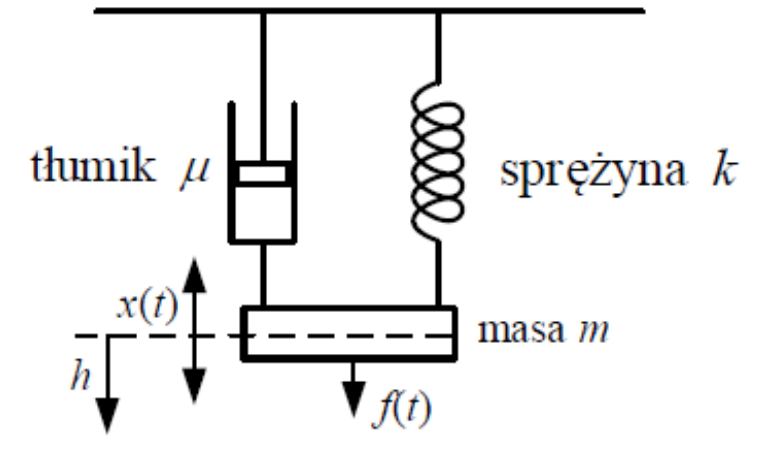
\includegraphics[width=\textwidth]{./img/schemat-1.png}
    \caption{Schemat układu z jednym tłumikiem i sprężyną}
    \label{schemat1}
  \end{minipage}
  \hfill
  \begin{minipage}[b]{0.4\textwidth}
    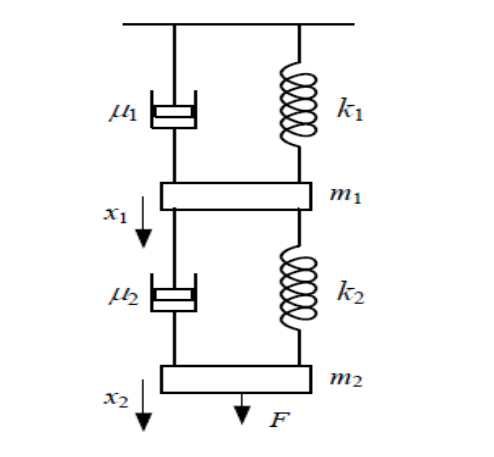
\includegraphics[width=\textwidth]{./img/schemat-2.png}
    \caption{Schemat układu podwójnego.}
    \label{schemat2}
  \end{minipage}
\end{figure}


\begin{table}[H]
\begin{tabular}{lllllllll}
\hline
\textbf{Numer} & \textbf{$m=m_1$} & \textbf{$m_2$} & \textbf{$u=u_1$} & \textbf{$u_2$} & \textbf{$k=k_1$} & \textbf{$k_2$} & \textbf{a} & \textbf{w} \\ \hline
13             & 1             & 5           & 6               & 1             & 4               & 1             & 2          & 1          \\ \hline
\end{tabular}
\caption{Parametry modelowanych układów}
\end{table}

Zostaną zbadane następujące siły zewnętrzne:
$$f_1 = a*sin(\omega t) $$ oraz
$$f_2 = a*e^{sin(\omega t)} $$
Przy wartościach początkowych dla pierwszego układu:
$$x(0) = 1, x'(0) = 0$$
$$x(0) = 1, x'(0) = 1$$
$$x(0) = 0, x'(0) = 1$$
A dla drugiego układu:
$$x_1(0)=1, x_1'(0)=0, x_1(0)=0, x_2'(0)=1 $$
$$x_1(0)=0, x_1'(0)=1, x_1(0)=1, x_2'(0)=0 $$
$$x_1(0)=1, x_1'(0)=1, x_1(0)=0, x_2'(0)=0 $$


\section{Rozwiązanie}

\subsection{Układ 1}

Układ pierwszy możemy rozwiązać analitycznie. Dla parametrów początkowych 
$x(0) = 1, x'(0) = 0$, wygląda to następująco:

\begin{figure}[H]
\centering
    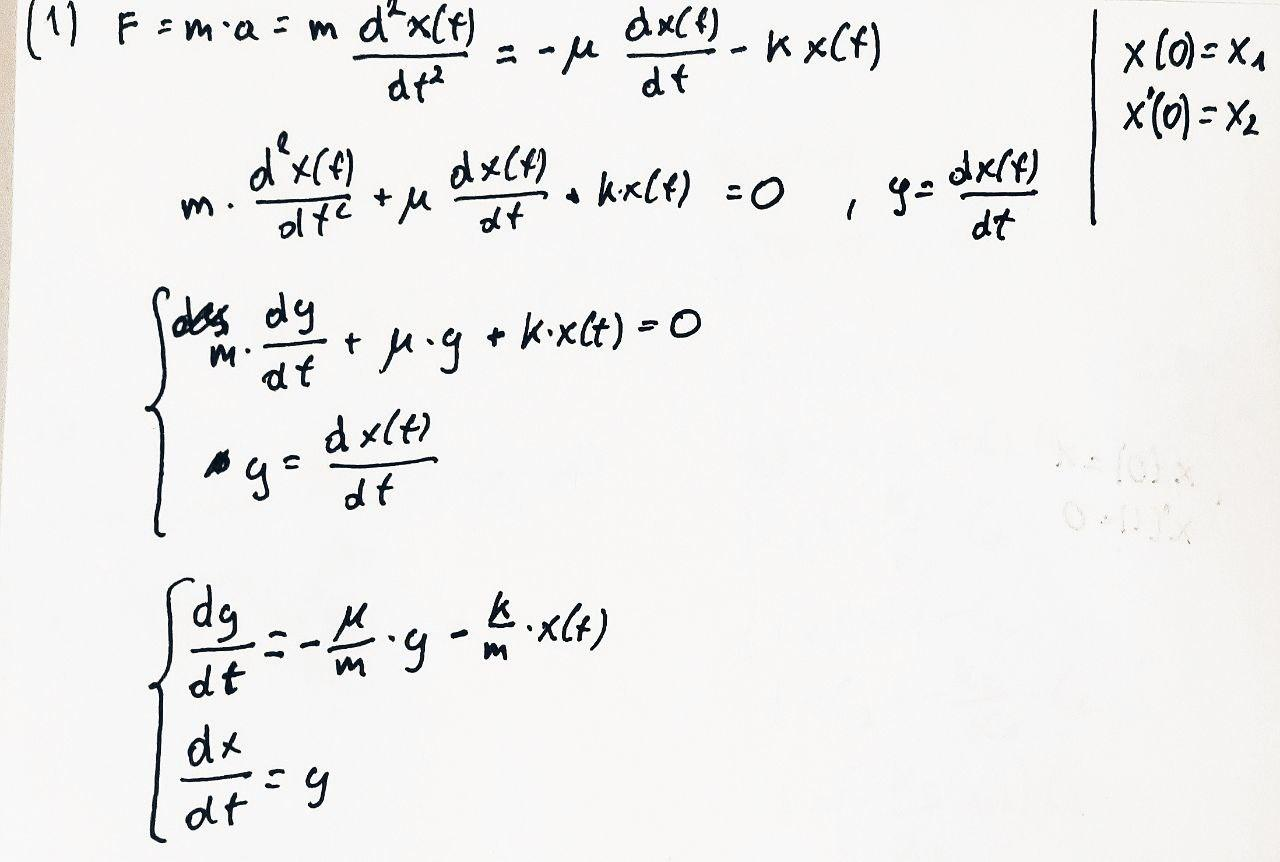
\includegraphics[scale=0.28]{./img/rozw-1.jpg}
\end{figure}

\begin{figure}[H]
\centering
    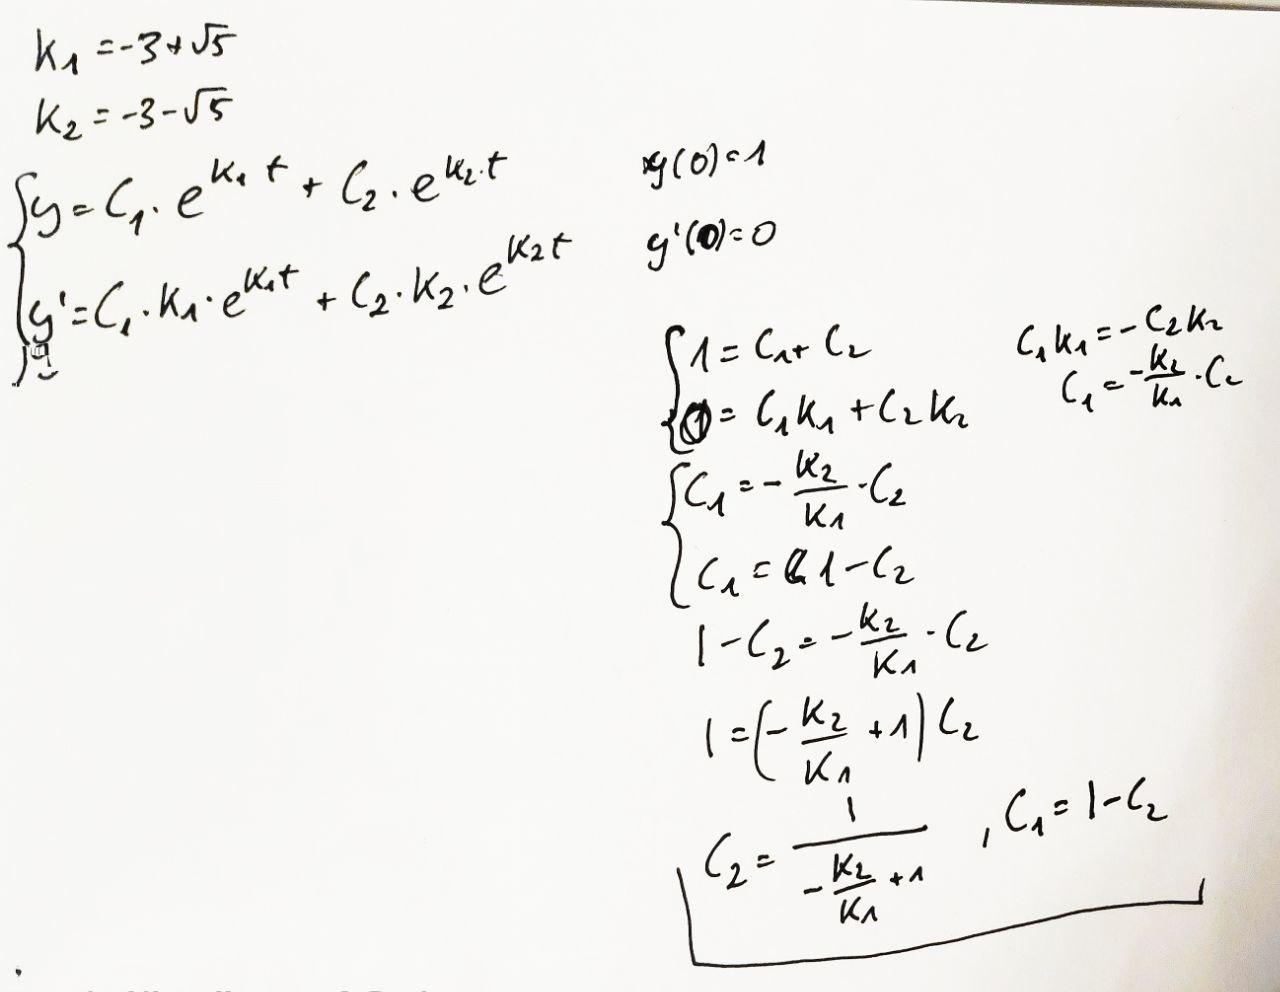
\includegraphics[scale=0.28]{./img/rozw-2.jpg}
\end{figure}

\subsubsection{Badanie typów rozwiązań}
Postać ogólna rozwiązywanego równania wygląda następująco:
$$ y'' + py' + qy = 0 $$
W zależności od tego, jakie przyjmiemy parametry, jego rozwiązanie zależy
od parametrów $k_1$ oraz $k_2$, gdzie:
$$k = -\frac{p}{2} \pm \sqrt{\frac{p^2}{4}-q}$$
Możliwe są zatem 3 przypadki:
\begin{enumerate}
    \item $k_1, k_2$ są rzeczywiste różne od siebie
    \item $k_1, k_2$ są zespolone
    \item $k_1, k_2$ są równe (rzeczywiste lub zespolone)
\end{enumerate}

\begin{lstlisting}[label={code1},language=scilab,caption={Kod generujący wykresy}]
function zad5(u, k, m, y0)
    for u = (u-0.1*u):0.05:(u+0.1*u)
        for k = (k-0.1*k):0.05:(k-0.1*k)
            for m = (m-0.1*m):0.05:(m-0.1*m)
                function dy=fun(t, y)
                    dy(1)=y(2);
                    dy(2)=-u/m*y(2)-k/m*y(1);
                endfunction
                
                t0=0.0;
                T=0.0:0.1:10;
                y=ode(y0,t0,T,fun,list(fun));
                scf(3);
                plot(T,y); xgrid();
                scf(4);
                plot(y(1,:),y(2,:)); xgrid();
            end
        end
    end
endfunction


zad5(6, 4, 1, [1;0]) // k_1 i k_2 są rozne, rzeczywiste
xs2png(3, "img/5-rzeczywiste-xy.png")
xs2png(4, "img/5-rzeczywiste-phase.png")
close();close();

zad5(1, 4, 1, [1;0]) // k_1 i k_2 są zespolone
xs2png(3, "img/5-zespolone-xy.png")
xs2png(4, "img/5-zespolone-phase.png")
close();close();

zad5(0, 4, 1, [1;0]) // k1 i k_2 brak oporu
xs2png(3, "img/5-boporu-xy.png")
xs2png(4, "img/5-boporu-phase.png")
close();close();

zad5(2, 4, 1, [1;0]) // k1 i k_2 są rowne
xs2png(3, "img/5-rowne-xy.png")
xs2png(4, "img/5-rowne-phase.png")
close();close();
\end{lstlisting}

\subsubsection{Rozwiązanie układu z modyfikacją parametrów przy $x(0)=1, x'(0)=0$}

\begin{figure}[H]
  \centering
  \hspace{-1.6cm}
  \begin{minipage}[b]{0.49\textwidth}
    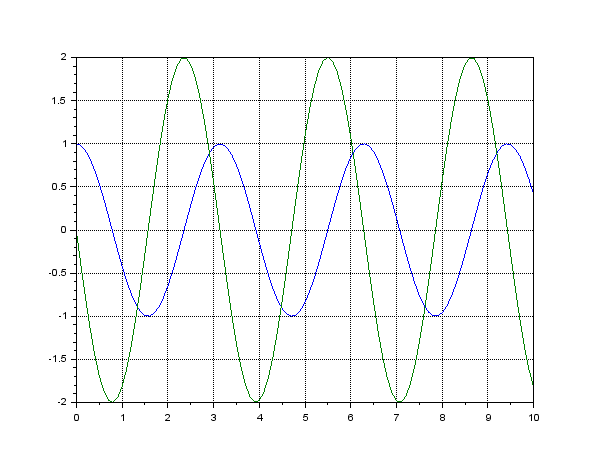
\includegraphics[scale=0.47]{./img/5-boporu-xy}
    \caption{Rozwiązanie \\ \centering$x''+4x=0$}
    \label{5-boporu-xy}
  \end{minipage}
  \hfill
  \begin{minipage}[b]{0.49\textwidth}
    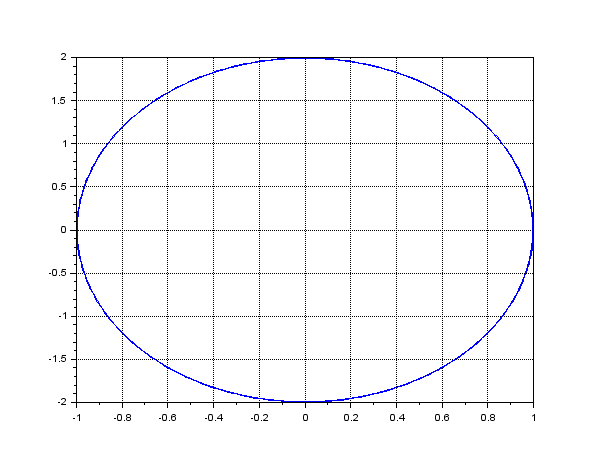
\includegraphics[scale=0.47]{./img/5-boporu-phase}
    \caption{Wykres fazowy \\ \centering$x''+4x=0$}
    \label{5-boporu-phase}
  \end{minipage}
\end{figure}

\begin{figure}[H]
  \centering
  \hspace{-1.6cm}
  \begin{minipage}[b]{0.49\textwidth}
    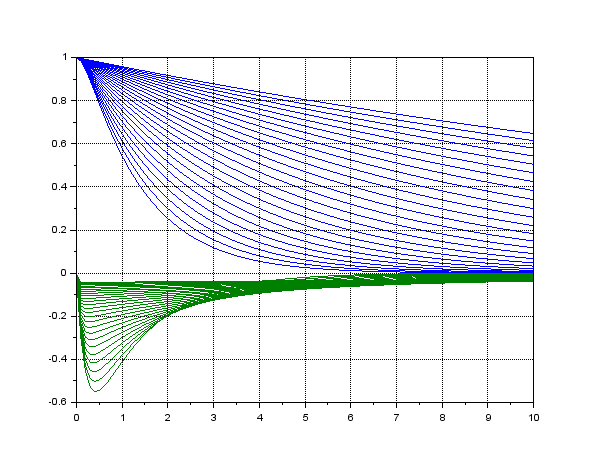
\includegraphics[scale=0.47]{./img/5-rzeczywiste-xy}
    \caption{Rozwiązanie \\ \centering$x''+6x'+4x=0$}
    \label{5-rzeczywiste-xy}
  \end{minipage}
  \hfill
  \begin{minipage}[b]{0.49\textwidth}
    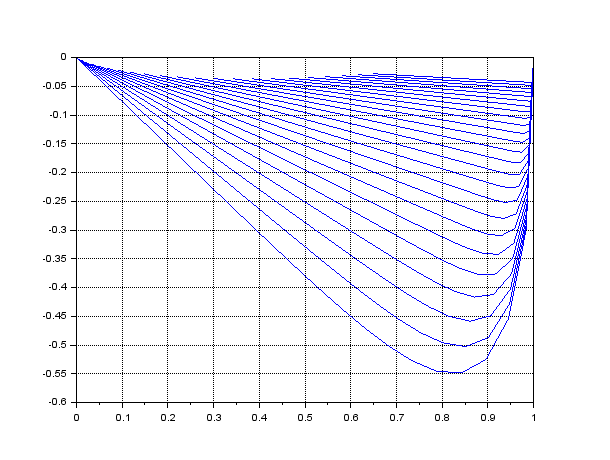
\includegraphics[scale=0.47]{./img/5-rzeczywiste-phase}
    \caption{Wykres fazowy \\ \centering$x''+6x'+4x=0$}
    \label{5-rzeczywiste-phase}
  \end{minipage}
\end{figure}

\begin{figure}[H]
  \centering
  \hspace{-1.6cm}
  \begin{minipage}[b]{0.49\textwidth}
    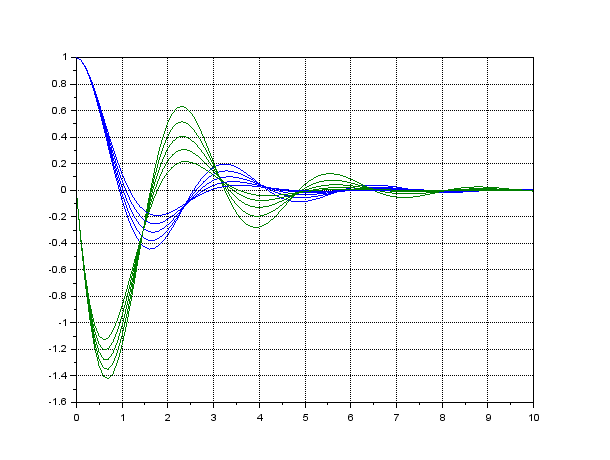
\includegraphics[scale=0.47]{./img/5-zespolone-xy}
    \caption{Rozwiązanie \\ \centering$x''+1x'+4x=0$}
    \label{5-zespolone-xy}
  \end{minipage}
  \hfill
  \begin{minipage}[b]{0.49\textwidth}
    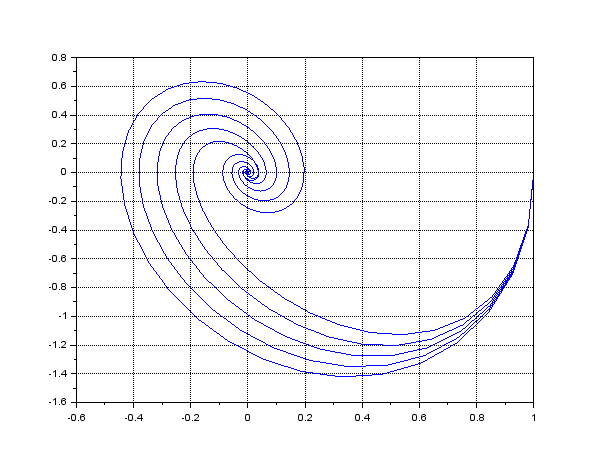
\includegraphics[scale=0.47]{./img/5-zespolone-phase}
    \caption{Wykres fazowy \\ \centering $x''+1x'+4x=0$}
    \label{5-zespolone-phase}
  \end{minipage}
\end{figure}

\begin{figure}[H]
  \centering
  \hspace{-1.6cm}
  \begin{minipage}[b]{0.49\textwidth}
    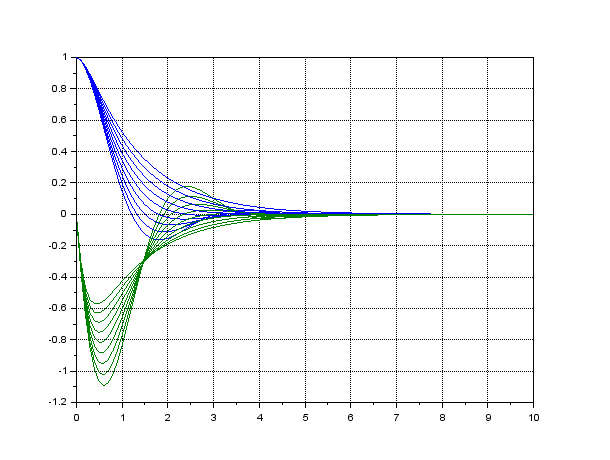
\includegraphics[scale=0.47]{./img/5-rowne-xy}
    \caption{Rozwiązanie \\ \centering $x''+2x'+4x=0$}
    \label{5-rowne-xy}
  \end{minipage}
  \hfill
  \begin{minipage}[b]{0.49\textwidth}
    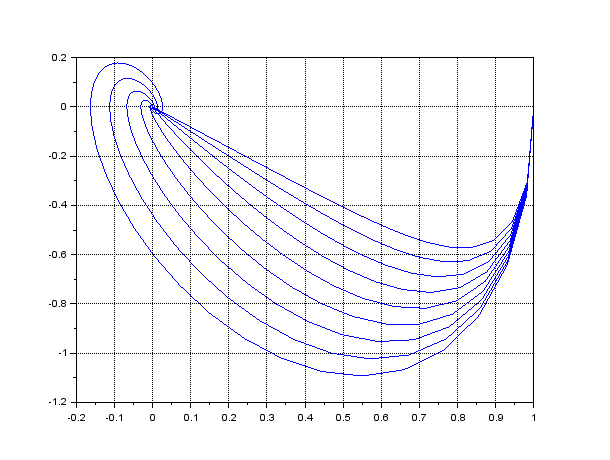
\includegraphics[scale=0.47]{./img/5-rowne-phase}
    \caption{Wykres fazowy \\
    \centering $x''+2x'+4x=0$}
    \label{5-rowne-phase}
  \end{minipage}
\end{figure}

\subsubsection{Rozwiązanie zadanego układu ze zmianą parametrów przy $x(0)=0, x'(0)=1$}

\begin{figure}[H]
  \centering
  \hspace{-1.6cm}
  \begin{minipage}[b]{0.49\textwidth}
    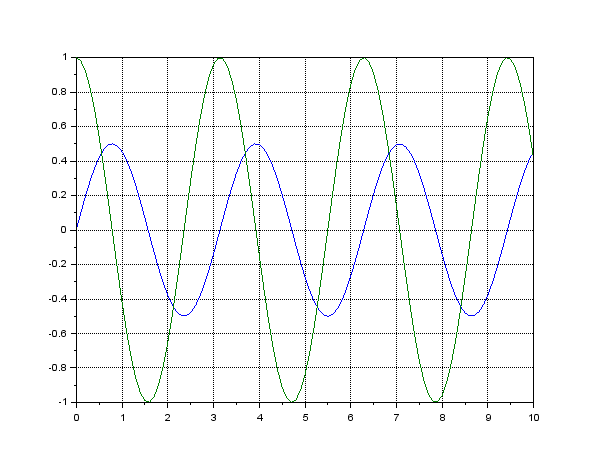
\includegraphics[scale=0.47]{./img/5-boporu-xy-01}
    \caption{Rozwiązanie \\ \centering $x''+2x'+4x=0$}
  \end{minipage}
  \hfill
  \begin{minipage}[b]{0.49\textwidth}
    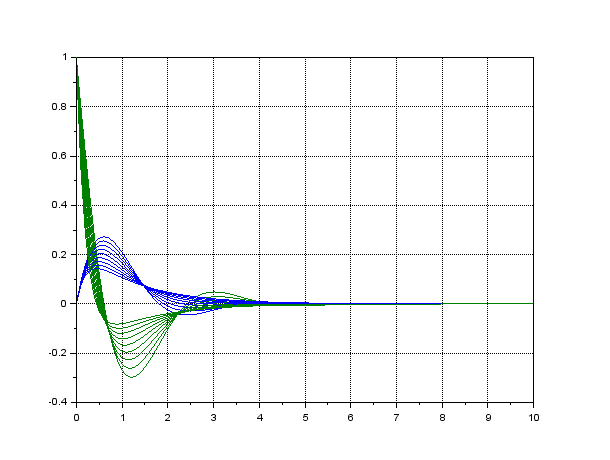
\includegraphics[scale=0.47]{./img/5-rowne-xy-01}
    \caption{Wykres fazowy \\
    \centering $x''+2x'+4x=0$}
  \end{minipage}
\end{figure}

\begin{figure}[H]
  \centering
  \hspace{-1.6cm}
  \begin{minipage}[b]{0.49\textwidth}
    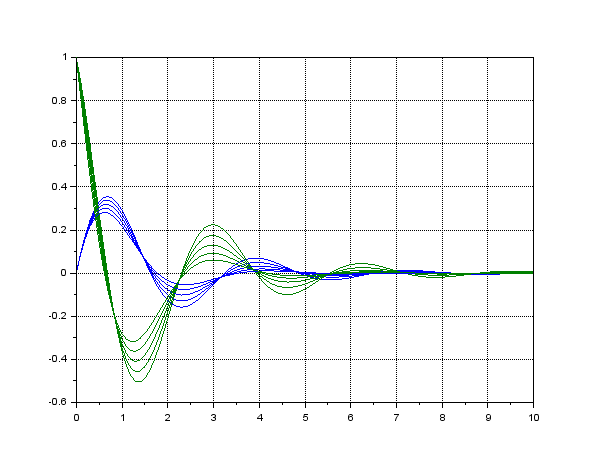
\includegraphics[scale=0.47]{./img/5-zespolone-xy-01}
    \caption{Rozwiązanie \\ \centering $x''+2x'+4x=0$}
  \end{minipage}
  \hfill
  \begin{minipage}[b]{0.49\textwidth}
    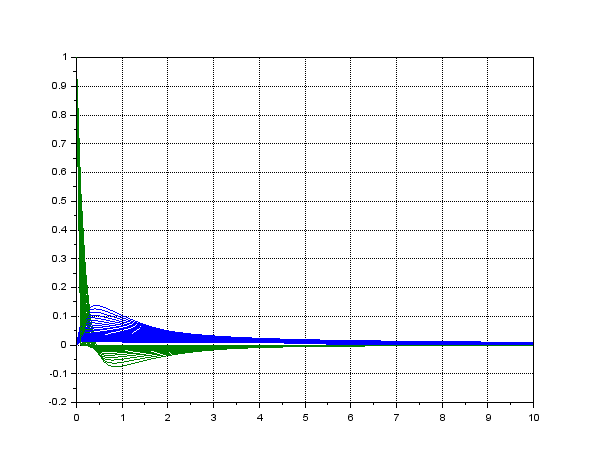
\includegraphics[scale=0.47]{./img/5-rzeczywiste-xy-01}
    \caption{Wykres fazowy \\
    \centering $x''+2x'+4x=0$}
  \end{minipage}
\end{figure}

\subsubsection{Rozwiązanie zadanego układu ze zmianą parametrów przy $x(0)=1, x'(0)=1$}

\begin{figure}[H]
  \centering
  \hspace{-1.6cm}
  \begin{minipage}[b]{0.49\textwidth}
    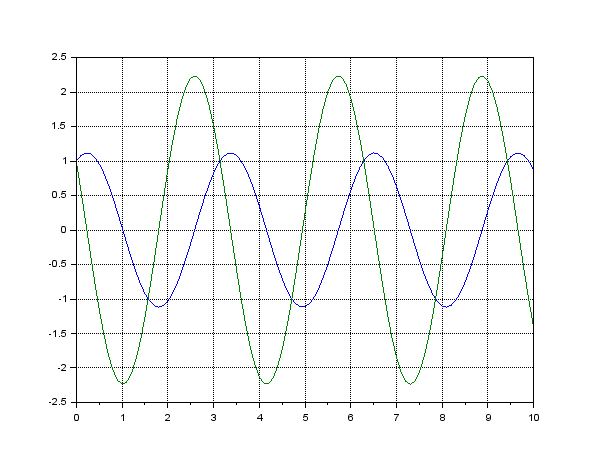
\includegraphics[scale=0.47]{./img/5-boporu-xy-11}
    \caption{Rozwiązanie \\ \centering $x''+2x'+4x=0$}
  \end{minipage}
  \hfill
  \begin{minipage}[b]{0.49\textwidth}
    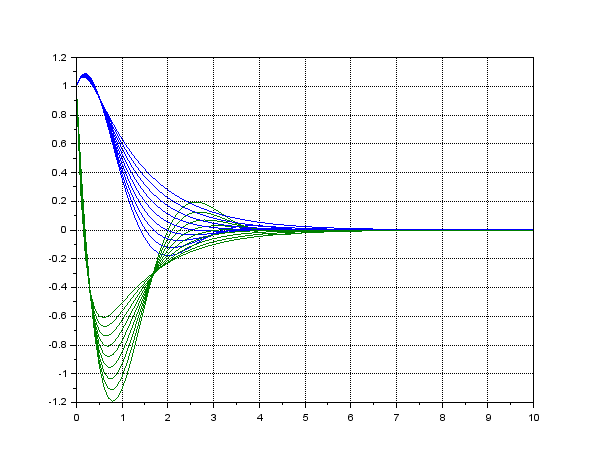
\includegraphics[scale=0.47]{./img/5-rowne-xy-11}
    \caption{Wykres fazowy \\
    \centering $x''+2x'+4x=0$}
  \end{minipage}
\end{figure}

\begin{figure}[H]
  \centering
  \hspace{-1.6cm}
  \begin{minipage}[b]{0.49\textwidth}
    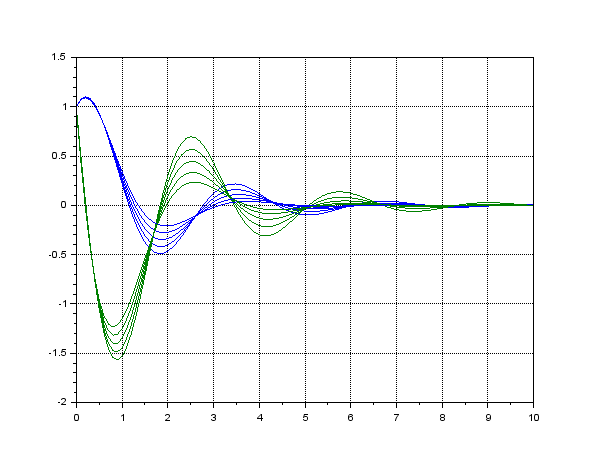
\includegraphics[scale=0.47]{./img/5-zespolone-xy-11}
    \caption{Rozwiązanie \\ \centering $x''+2x'+4x=0$}
  \end{minipage}
  \hfill
  \begin{minipage}[b]{0.49\textwidth}
    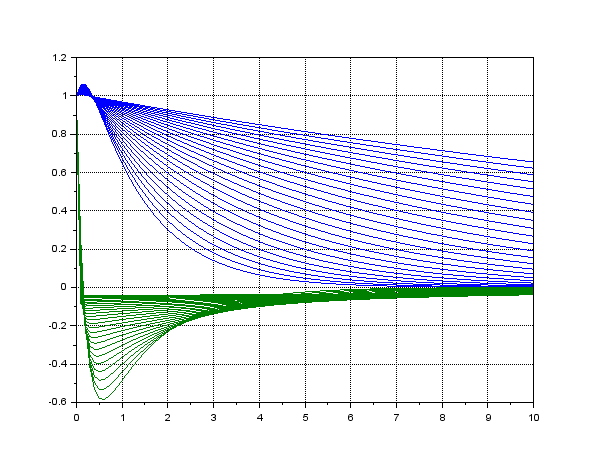
\includegraphics[scale=0.47]{./img/5-rzeczywiste-xy-11}
    \caption{Wykres fazowy \\
    \centering $x''+2x'+4x=0$}
  \end{minipage}
\end{figure}

\null\hfill Piotr Krawiec
\end{document}